In this section, we illustrate the performance of the standard and variance deconvolution Saltelli SI estimators. 
We first discuss results for a common GSA numerical example -- the Ishigami function.
Then, we test the method on a Monte Carlo radiation transport problem.

We consider the Ishigami function~\cite{ishigami-homma-1990} as a case in which the true solution for $Q(\xi)$, $\Vxi{Q}$, and the full set of first- and total-order estimators is known:
\begin{gather}
    Q(\xi) = \sin \left( \xi_1 \right) + 7 \sin^2 \left( \xi_2 \right) + 0.1 \xi_3^4 \sin \left( \xi_1 \right) ,
\end{gather}
where the input parameters are independently uniformly distributed over $\left[-\pi, \pi\right]$.
We introduce stochasticity to the problem by adding a random variable $\eta \sim \mathcal{N} \left[0,1\right]$ multiplied by a constant,
\begin{equation}
    f(\xi,\eta) = Q(\xi) + c \eta ,
\end{equation}
and approximate $Q(\xi)$ as $\Qpoll(\xi)$ using MC.  
This results in a total variance 
\begin{equation}
    \Var{\Qpoll} = \Vxi{Q} + \frac{c^2}{\Neta},
\end{equation}
where $\Vxi{Q}=13.84$ is the known variance of the Ishigami function.
The expected value of the Ishigami function is $\EExi{Q} = 3.5$.
The behavior of the Ishigami indices is also known: $\xi_1$ and $\xi_3$ are highly interactive while $\xi_2$ is purely additive, i.e., $\S{2} = \T{2}$, and $\S{3}=0$.
This allows us to observe the behavior of the variance deconvolution estimators under both purely additive and highly-interactive model conditions, as well as their behavior when an index is equal to zero, which can cause estimator performance to suffer.
In this exercise, we numerically compare the performance of the standard estimators (Eqs.~\eqref{eq:saltelli-si-poll} and~\eqref{eq:saltelli-ti-poll}) with the performance of the variance deconvolution estimators (Eqs.~\eqref{eq:saltelli-si-vard} and~\eqref{eq:saltelli-ti-vard}).
Changing the constant $c$ allows us to control how much the solver noise contributes to the total variance and how much resolution is needed in $\Neta$.
We compare their behavior for multiple combinations of $(\Nxi, \Neta)$ and replicate one hundred estimates of the first- and total-order indices using the procedure laid out in Section~\ref{sec:sampling}.
We note again that we are sampling the parameter space using purely random MC.

\subsubsection{Equal solver and parameter noise}
We first consider the case in which $c=3.721$, such that the solver noise contributes about $50\%$ of the variance of a single tally $f$.
In Figures~\ref{fig:mediumc-eta100-si} and~\ref{fig:mediumc-eta100-ti}, we show boxplots of the 100 replicates of first- and total-order Sobol’ indices (respectively), where the boxplot represents the minimum, first-quartile, median, third-quartile and maximum, plus the mean in a dotted line.
We see that the solver noise has been resolved out with $\Neta=100$ solver samples and the standard and variance deconvolution estimators have both converged to the true indices with similar variances. 
For the boxplots in Figures~\ref{fig:mediumc-eta2-si} and~\ref{fig:mediumc-eta2-ti}, we have reduced the solver sample size to $\Neta=2$, a 50X reduction in total cost. 
For $\S{1}$ and $\S{2}$, we see that the variance deconvolution estimator has a similar spread as the standard estimator, but the standard estimator's bias is such that the true value is outside the first quartile.
As predicted, the bias of the standard estimator underestimates the true first-order indices.
Both estimators accurately find $\S{3}=0$, however, we see that the variance deconvolution estimator has a larger variability than the standard estimator.
For all three total-order indices, the bias of the standard estimator overestimates the true indices; for $\T{2}$ and $\T{3}$, the true value is entirely outside of the boxplot.
The decrease in computational cost did affect the variance deconvolution estimator; for $\T{1}$ in particular, we see that while the variance deconvolution estimator is unbiased, its variability is has increased and is larger than that of the standard estimator.
In $\T{3}$, we see that the low-resolution estimate of the solver variance has caused the variance deconvolution to, in essence, over-correct.

\begin{figure}
    \centering
    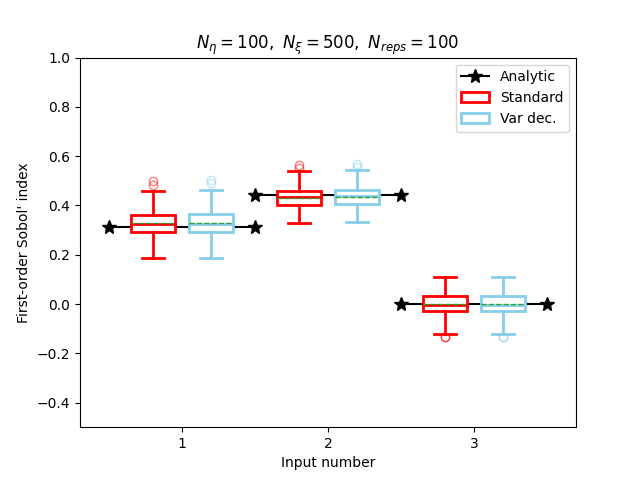
\includegraphics{figures/medium_c/si_eta100_xi500.png}
    \caption{Boxplot of the 100 replicates of first-order Sobol’ indices, where the solver noise is approx. equal to the parameter noise. The boxplot represents the minimum, first-quartile, median, third-quartile and maximum, plus the mean with a dotted line.}
    \label{fig:mediumc-eta100-si}
\end{figure}
\begin{figure}
    \centering
    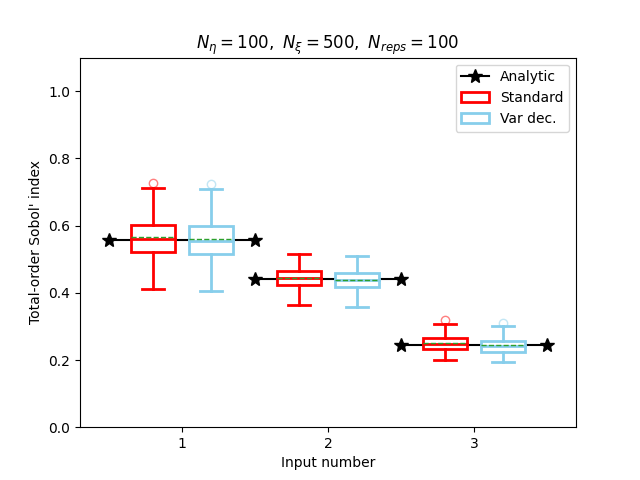
\includegraphics{figures/medium_c/ti_eta100_xi500.png}
    \caption{Boxplot of the 100 replicates of first-order Sobol’ indices, where the solver noise is approx. equal to the parameter noise. The boxplot represents the minimum, first-quartile, median, third-quartile and maximum, plus the mean with a dotted line.}
    \label{fig:mediumc-eta100-ti}
\end{figure}

\begin{figure}
    \centering
    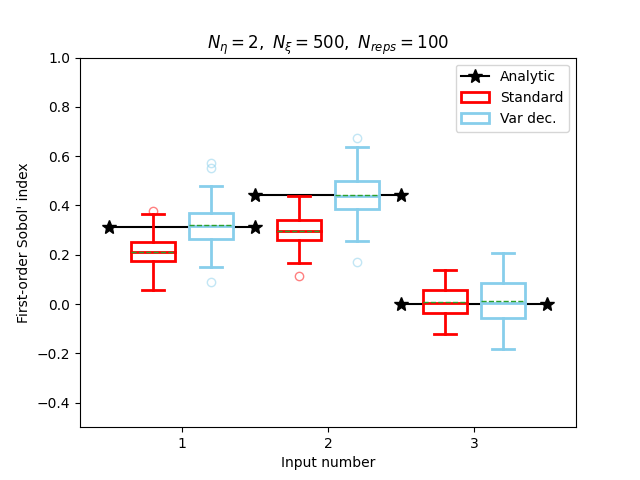
\includegraphics{figures/medium_c/si_eta2_xi500.png}
    \caption{Boxplot of the 100 replicates of first-order Sobol’ indices, where the solver noise is approx. equal to the parameter noise. The boxplot represents the minimum, first-quartile, median, third-quartile and maximum, plus the mean with a dotted line.}
    \label{fig:mediumc-eta2-si}
\end{figure}
\begin{figure}
    \centering
    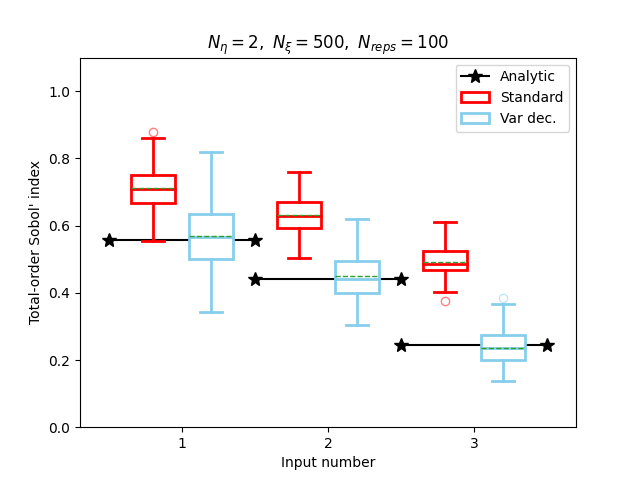
\includegraphics{figures/medium_c/ti_eta2_xi500.png}
    \caption{Boxplot of the 100 replicates of first-order Sobol’ indices, where the solver noise is approx. equal to the parameter noise. The boxplot represents the minimum, first-quartile, median, third-quartile and maximum, plus the mean with a dotted line.}
    \label{fig:mediumc-eta2-ti}
\end{figure}

\subsubsection{Solver noise is double parameter noise}
We now consider the case in which $c=5.3$, such that the solver noise contributes about $67\%$ of the variance of a single tally $f$.
In this case, more solver samples are required to produce unbiased indices using the standard estimators; in Figures~\ref{fig:largec-eta500-si} and~\ref{fig:largec-eta500-ti}, $\Neta=500$ were used, producing nearly identical results from the standard and variance deconvolution estimators.

In Figures~\ref{fig:largec-eta2-si} and~\ref{fig:largec-eta2-ti}, we again use the minimum number of solver samples $\Neta=2$, now a 250X reduction in cost. This produces large biases in the standard estimator and large variabilities and some over-correction in the variance deconvolution estimator.

Finally, in Figures~\ref{fig:largec-eta10-si} and~\ref{fig:largec-eta10-ti}, we use $\Neta=10$ solver samples, a 50X reduction from the well-resolved $\Neta=500$.
The variance deconvolution estimator is no longer over-correcting and is accurately computing all indices with a variability similar to that of the standard estimator.
For all indices except $\S{3}$, bias is still largely affecting the standard estimator.

\begin{figure}
    \centering
    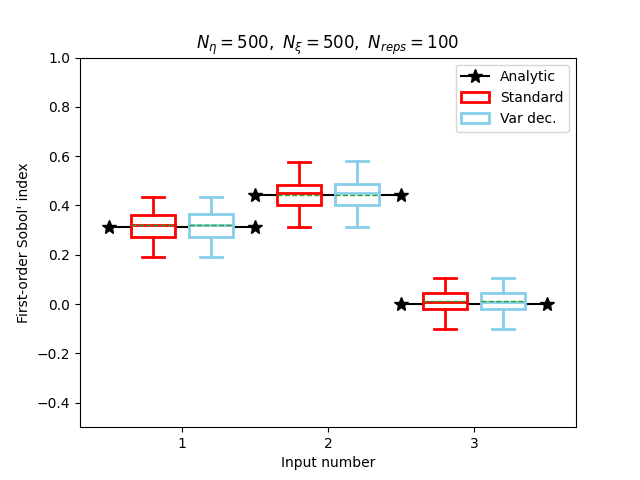
\includegraphics{figures/large_c/si_eta500_xi500.png}
    \caption{Boxplot of the 100 replicates of first-order Sobol’ indices, where the solver noise is approx. double the parameter noise. The boxplot represents the minimum, first-quartile, median, third-quartile and maximum, plus the mean with a dotted line.}
    \label{fig:largec-eta500-si}
\end{figure}
\begin{figure}
    \centering
    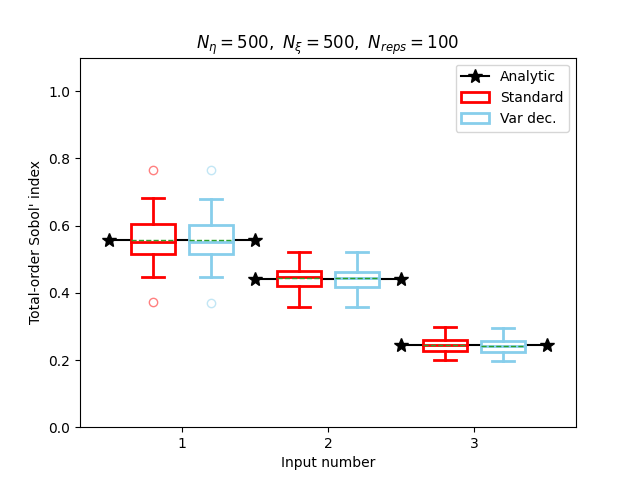
\includegraphics{figures/large_c/ti_eta500_xi500.png}
    \caption{Boxplot of the 100 replicates of first-order Sobol’ indices, where the solver noise is approx. double the parameter noise. The boxplot represents the minimum, first-quartile, median, third-quartile and maximum, plus the mean with a dotted line.}
    \label{fig:largec-eta500-ti}
\end{figure}


\begin{figure}
    \centering
    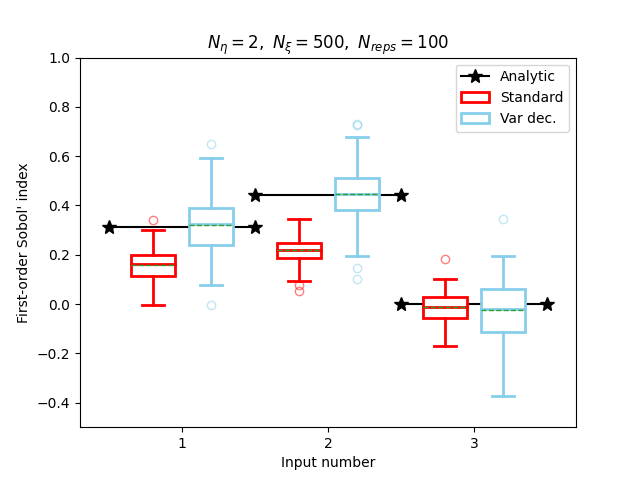
\includegraphics{figures/large_c/si_eta2_xi500.png}
    \caption{Boxplot of the 100 replicates of first-order Sobol’ indices, where the solver noise is approx. double the parameter noise. The boxplot represents the minimum, first-quartile, median, third-quartile and maximum, plus the mean with a dotted line.}
    \label{fig:largec-eta2-si}
\end{figure}
\begin{figure}
    \centering
    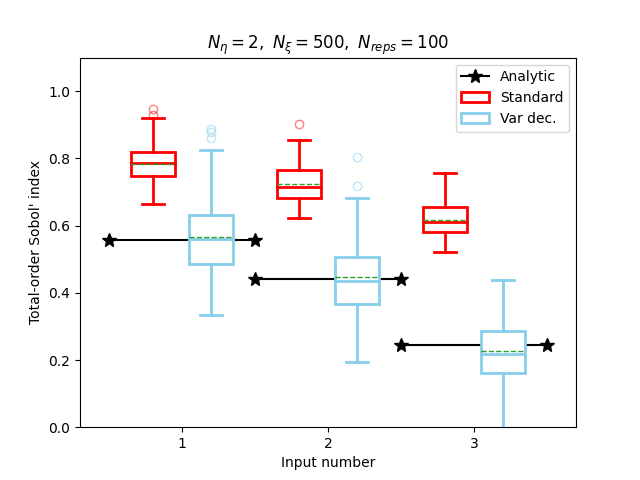
\includegraphics{figures/large_c/ti_eta2_xi500.png}
    \caption{Boxplot of the 100 replicates of first-order Sobol’ indices, where the solver noise is approx. double the parameter noise. The boxplot represents the minimum, first-quartile, median, third-quartile and maximum, plus the mean with a dotted line.}
    \label{fig:largec-eta2-ti}
\end{figure}

\begin{figure}
    \centering
    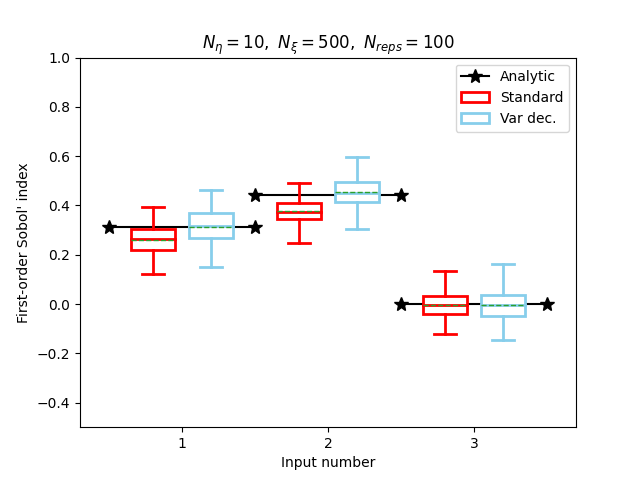
\includegraphics{figures/large_c/si_eta10_xi500.png}
    \caption{Boxplot of the 100 replicates of first-order Sobol’ indices, where the solver noise is approx. double the parameter noise. The boxplot represents the minimum, first-quartile, median, third-quartile and maximum, plus the mean with a dotted line.}
    \label{fig:largec-eta10-si}
\end{figure}
\begin{figure}
    \centering
    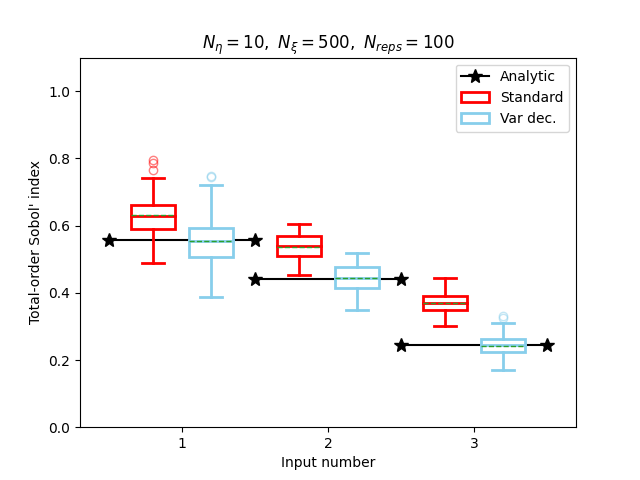
\includegraphics{figures/large_c/ti_eta10_xi500.png}
    \caption{Boxplot of the 100 replicates of first-order Sobol’ indices, where the solver noise is approx. double the parameter noise. The boxplot represents the minimum, first-quartile, median, third-quartile and maximum, plus the mean with a dotted line.}
    \label{fig:largec-eta10-ti}
\end{figure}


\subsection{Radiation transport test problem}
We next perform GSA on a contrived neutron transport problem solved using Monte Carlo radiation transport methods~\cite{lux-koblinger-90}. 
The problem is one-dimensional in space and steady-state in time, with the neutron energy spectrum is divided into 7 energy groups.
The problem has three components that make up a repeating lattice: a spatially-homogenized uranium dioxide (UO$_2$) fuel pin, water moderator, and a spatially homogenized control rod. 
There is an isotropic source, uniform in energy across all groups, at the spatial halfway point.
We use multi-group cross sections and geometry specifications from C5G7, a nuclear reactor benchmark developed by OECD/NEA~\cite{c5g7-2005}. 
In recent work, we tested the developed estimators on the full two-dimensional C5G7 benchmark; for more detail, see~\cite{clements-mc-2025}.

To test a wide spectrum of physics behavior, we introduce large parameter uncertainty to five independent factors. 
The densities of the fuel (1), the moderator (2), and the control rod (3) vary uniformly $\pm 70\%$ around their respective means; the ratio of fuel-diameter to moderator-diameter (4) ; and the diameter of the control rod (5) varies uniformly between 0.2 and 0.8. 
We define two quantities of interest as a function of space: the scalar flux integrated over the first two energy groups $\phi_F (x)$, and the scalar flux integrated over the remaining five energy groups $\phi_S(x)$.

For reference, using $\Nxi=5 \times 10^5$ and $\Neta=10^5$, Figure~\ref{fig:flux} shows $\phi_F (x)$ and $\phi_S (x)$. Figure~\ref{fig:indices} shows the full set of first- and total-order indices for both QoIs.
At this high $\Neta$, as expected, we see that $\pollSsalt{i}$ and $\pollTsalt{i}$ converge respectively to $\unpollSsalt{i}$ and $\unpollTsalt{i}$, causing their lines to overlap.
The faster group flux $\phi_F$ is most sensitive throughout the spatial domain to the density of the moderator ($\xi_2$), which is understandable as the density of the moderator will greatly impact the number of neutrons and their energies everywhere in the problem. 
The control rod's density ($\xi_3$) and thickness ($\xi_5$) are most impactful for the slower group flux, $\phi_S(x)$, with both having large inflection points at the nominal moderator--control rod boundary at $x=1.5$.
This is understandable, as the control rod is a primarily thermal absorber.

\begin{figure}[ht]
    \centering
    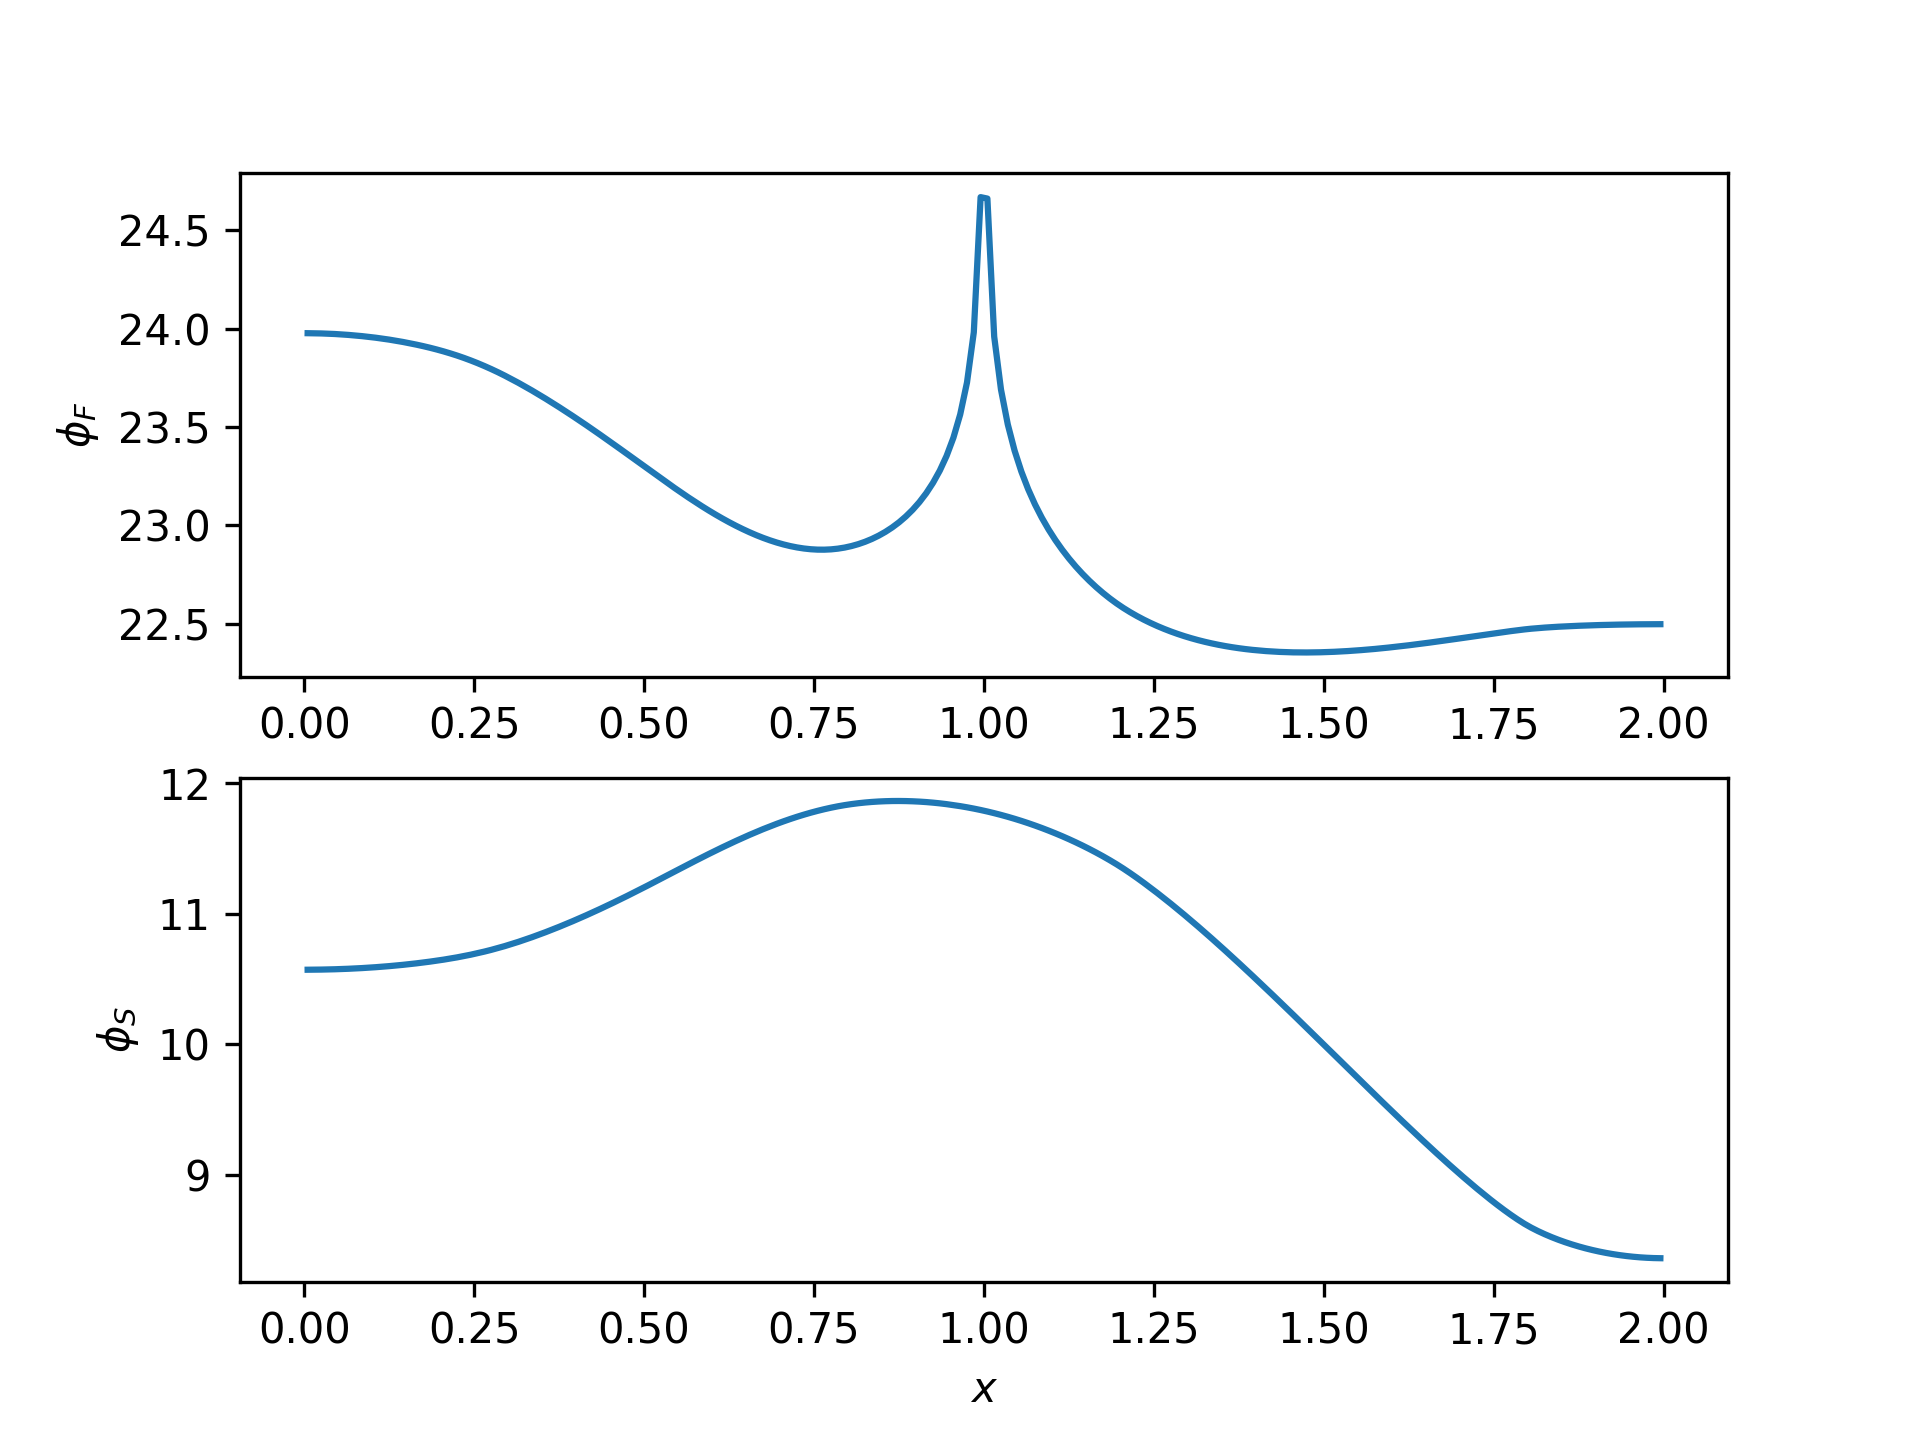
\includegraphics{figures/flux.png} 
    \caption{Average scalar flux with five uncertain parameters using $\Nxi=5 \times 10^5$, $\Neta=10^5$.}
    \label{fig:flux}
\end{figure}

\begin{figure}[ht]
    \centering
    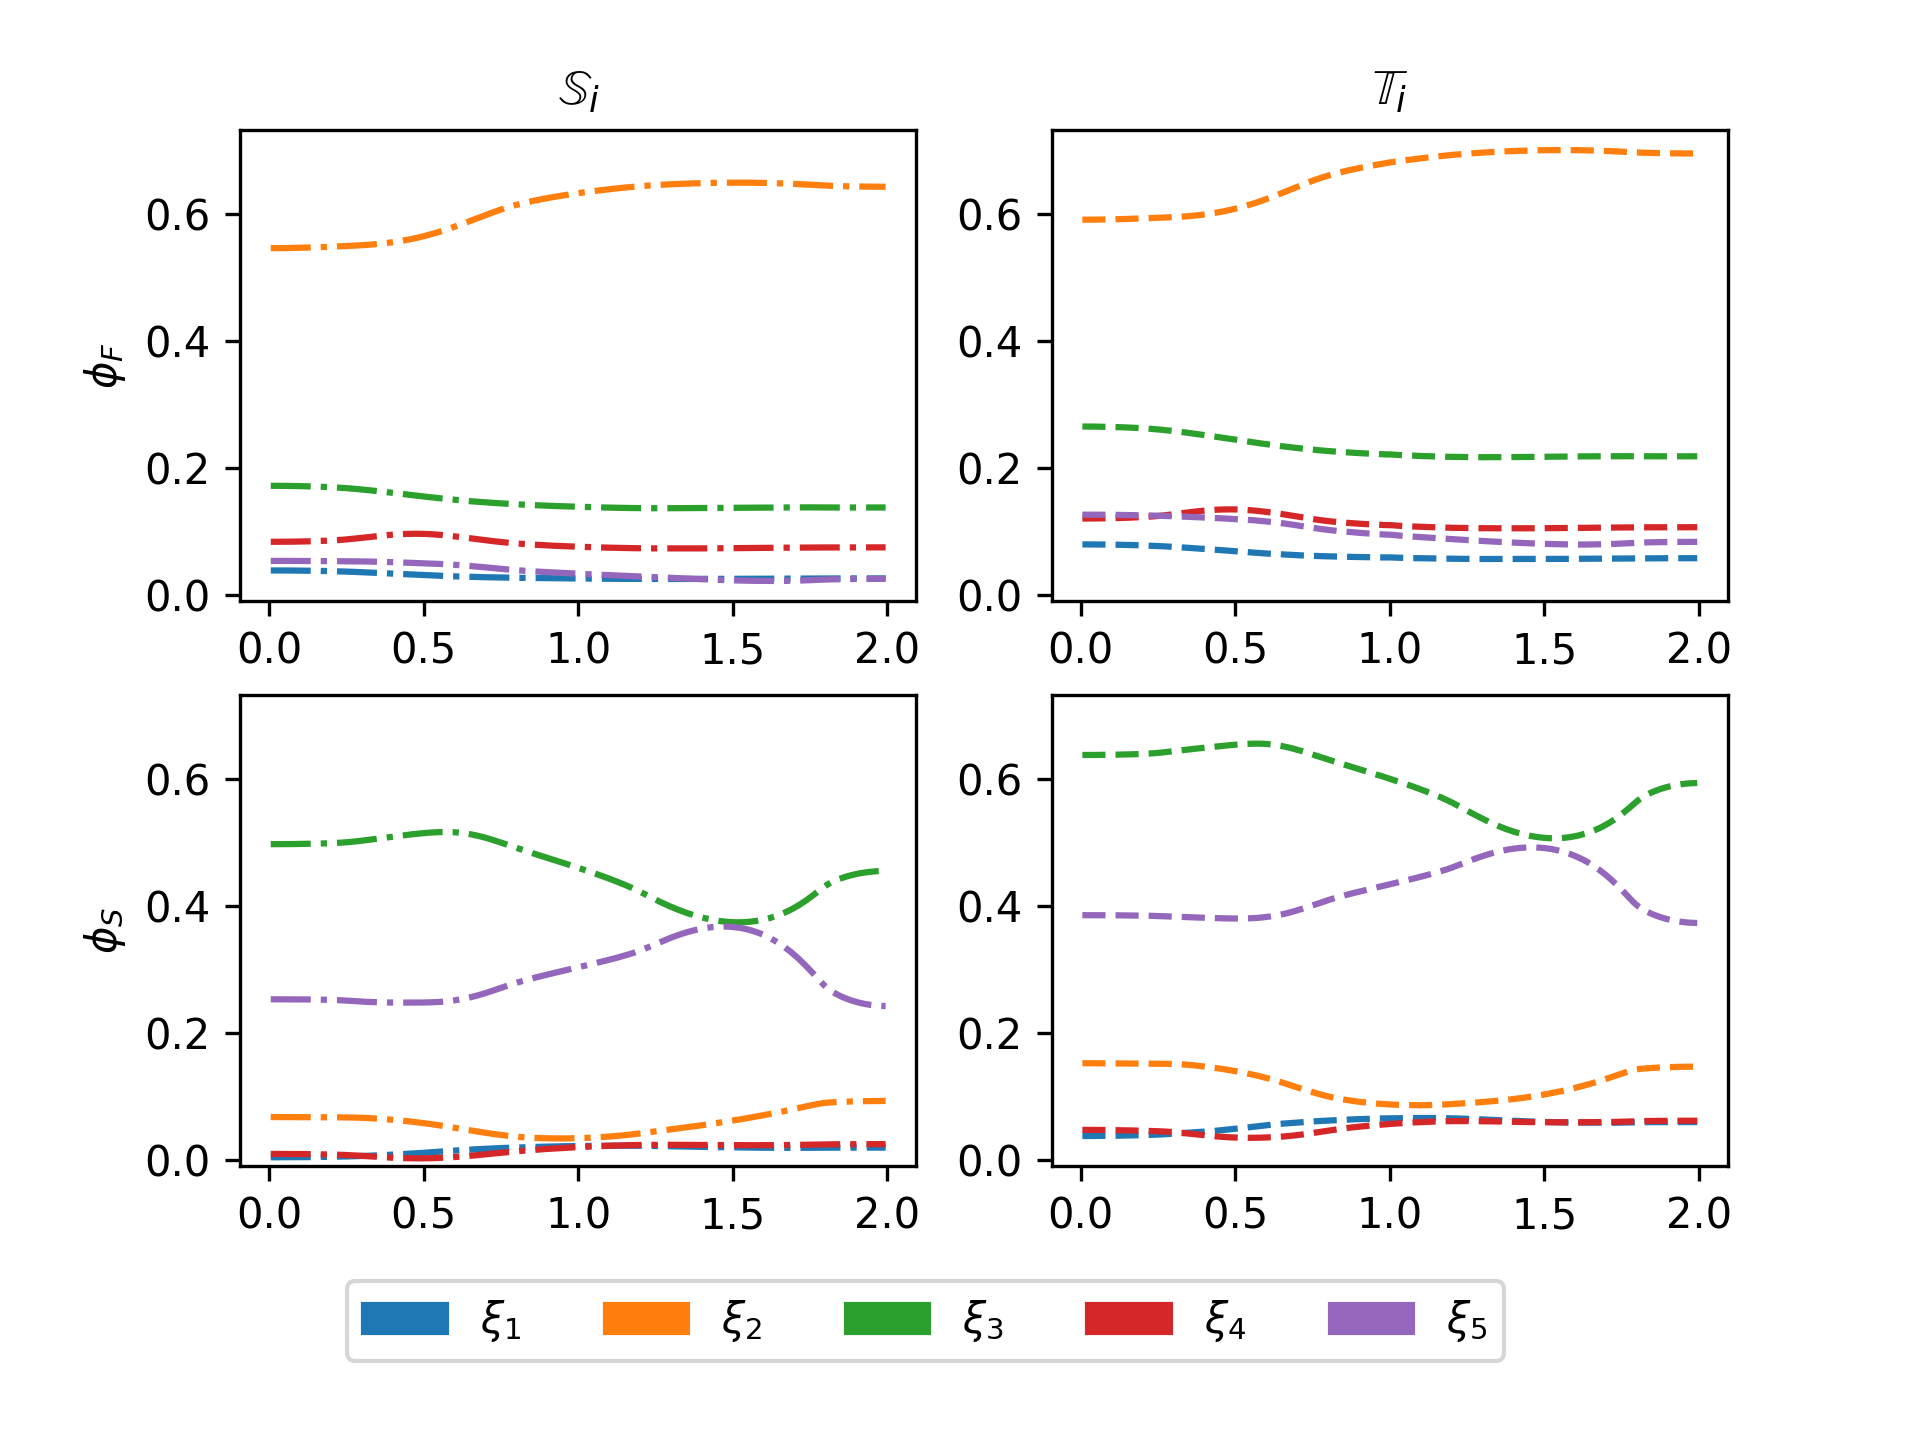
\includegraphics{figures/indices.png}
    \caption{Full set of first- and total- order indices of $\phi_F$ and $\phi_S$ using $\Nxi=5 \times 10^5$, $\Neta=10^5$. Standard and corrected estimators exactly overlap. Uncertain factors: the densities of 1) the fuel, 2) the moderator, 3) and the control rod were allowed to vary uniformly $\pm 70\%$; 4) the ratio of fuel-width to moderator-width and 5) the control-rod thickness were both allowed to vary uniformly between 0.2 and 0.8. }
    \label{fig:indices}
\end{figure}

To see the effect of the variance deconvolution correction, we compare the MSE of the standard and corrected estimators.
In Figure~\ref{fig:mse-fo-fast}, we consider a constant computational cost $\C = \left( \Nxi \times \Neta \right) = 5 \times 10^5$ in two different combinations of $\Nxi$ and $\Neta$.
In the first combination, $\left( \Nxi, \Neta \right) = \left( 5 \times 10^3, 10^2 \right)$, we see that the MSE of the standard estimator is clearly lower than that of the variance deconvolution estimator for $\S{1}$ and $\S{5}$. 
Both of these indices are very close to zero (see Figure~\ref{fig:indices}); in this case, the higher variance of the variance deconvolution estimator outweighs the bias of the standard estimator.
In the second combination, we have increased $\Nxi$ by a factor of 10 and decreased $\Neta$ by the same factor to keep $\C$ constant.
The variance deconvolution estimator benefits from this configuration, with a MSE that is lower than that of the standard estimator at most locations in $x$. 

This pattern is consistent across QoIs: when indices are close to zero the variance of the variance deconvolution estimator can outweigh the bias of the standard estimator, and for a constant $\C$ the variance deconvolution estimator generally benefits from increasing the $\Nxi$ at the expense of decreasing $\Neta$. 
In Figure~\ref{fig:mse-fo-slow}, we see this for $\S{i} \left[ \phi_S \right]$.
For estimating $\T{i}$, the correction in both the numerator and denominator makes the difference between the standard and variance deconvolution estimators more drastic.
In Figures~\ref{fig:mse-to-fast} and~\ref{fig:mse-to-slow}, we see that the variance deconvolution estimator outperforms the standard across $x$ for both $\phi_F$ and $\phi_S$.

\begin{figure}
    \centering
    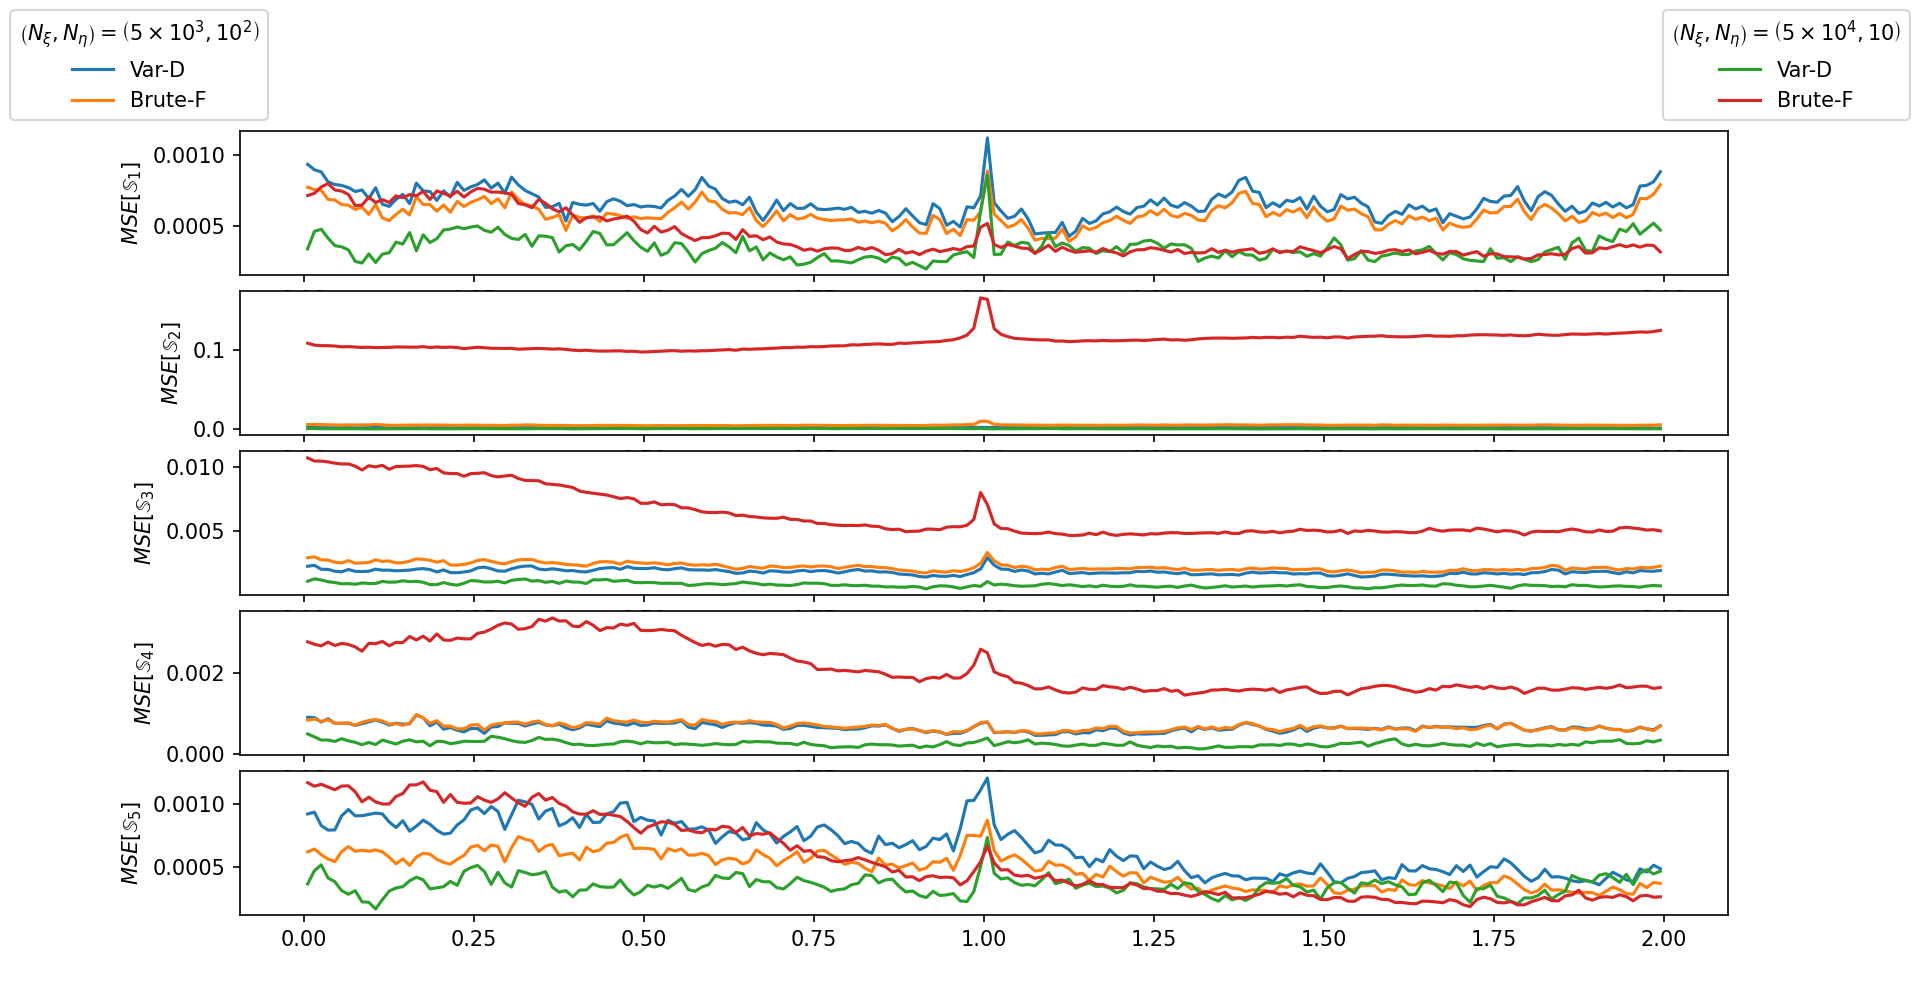
\includegraphics[width=\textwidth]{figures/mse_firstorder_fast.png}
    \caption{$MSE\left[\S{i}\right]$ for $\phi_F$, constant computational cost $\C = \left( \Nxi \times \Neta \right) = 5 \times 10^5$.}
    \label{fig:mse-fo-fast}
\end{figure}

\begin{figure}
    \centering
    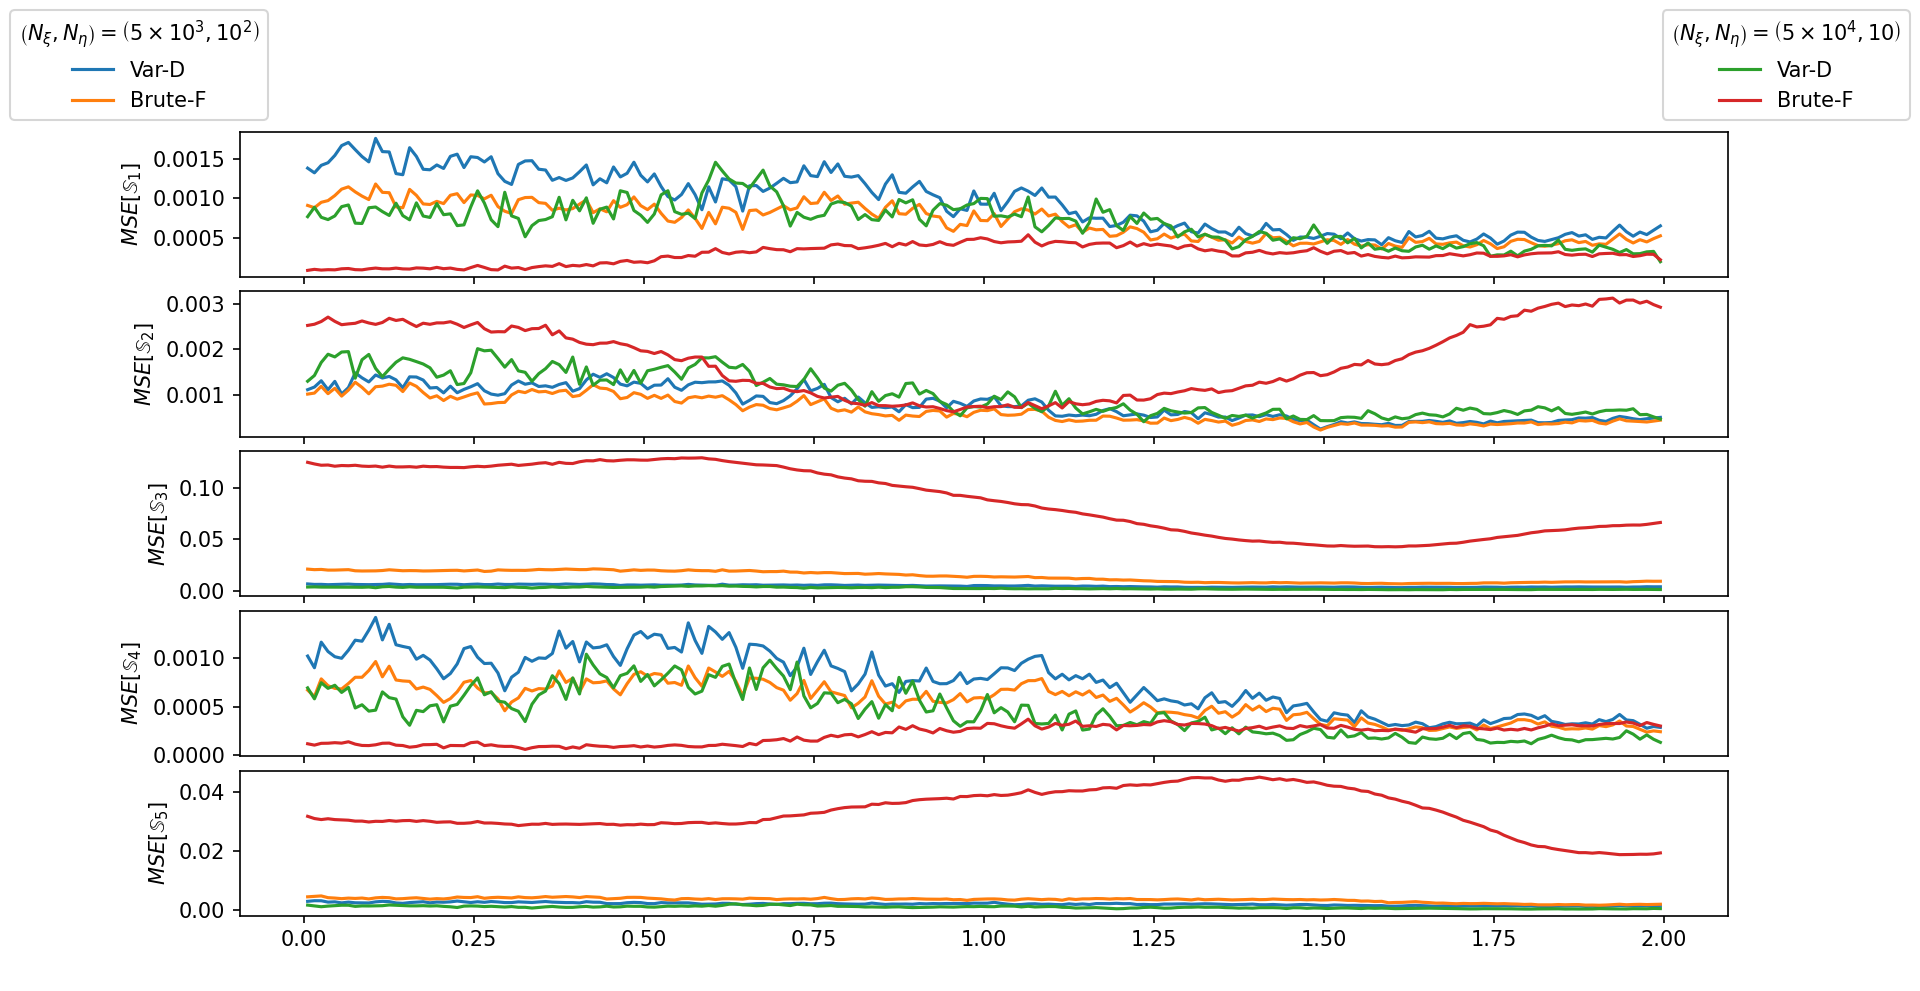
\includegraphics[width=\textwidth]{figures/mse_firstorder_slow.png}
    \caption{$MSE\left[\S{i}\right]$ for $\phi_S$, constant computational cost $\C = \left( \Nxi \times \Neta \right) = 5 \times 10^5$.}
    \label{fig:mse-fo-slow}
\end{figure}

\begin{figure}
    \centering
    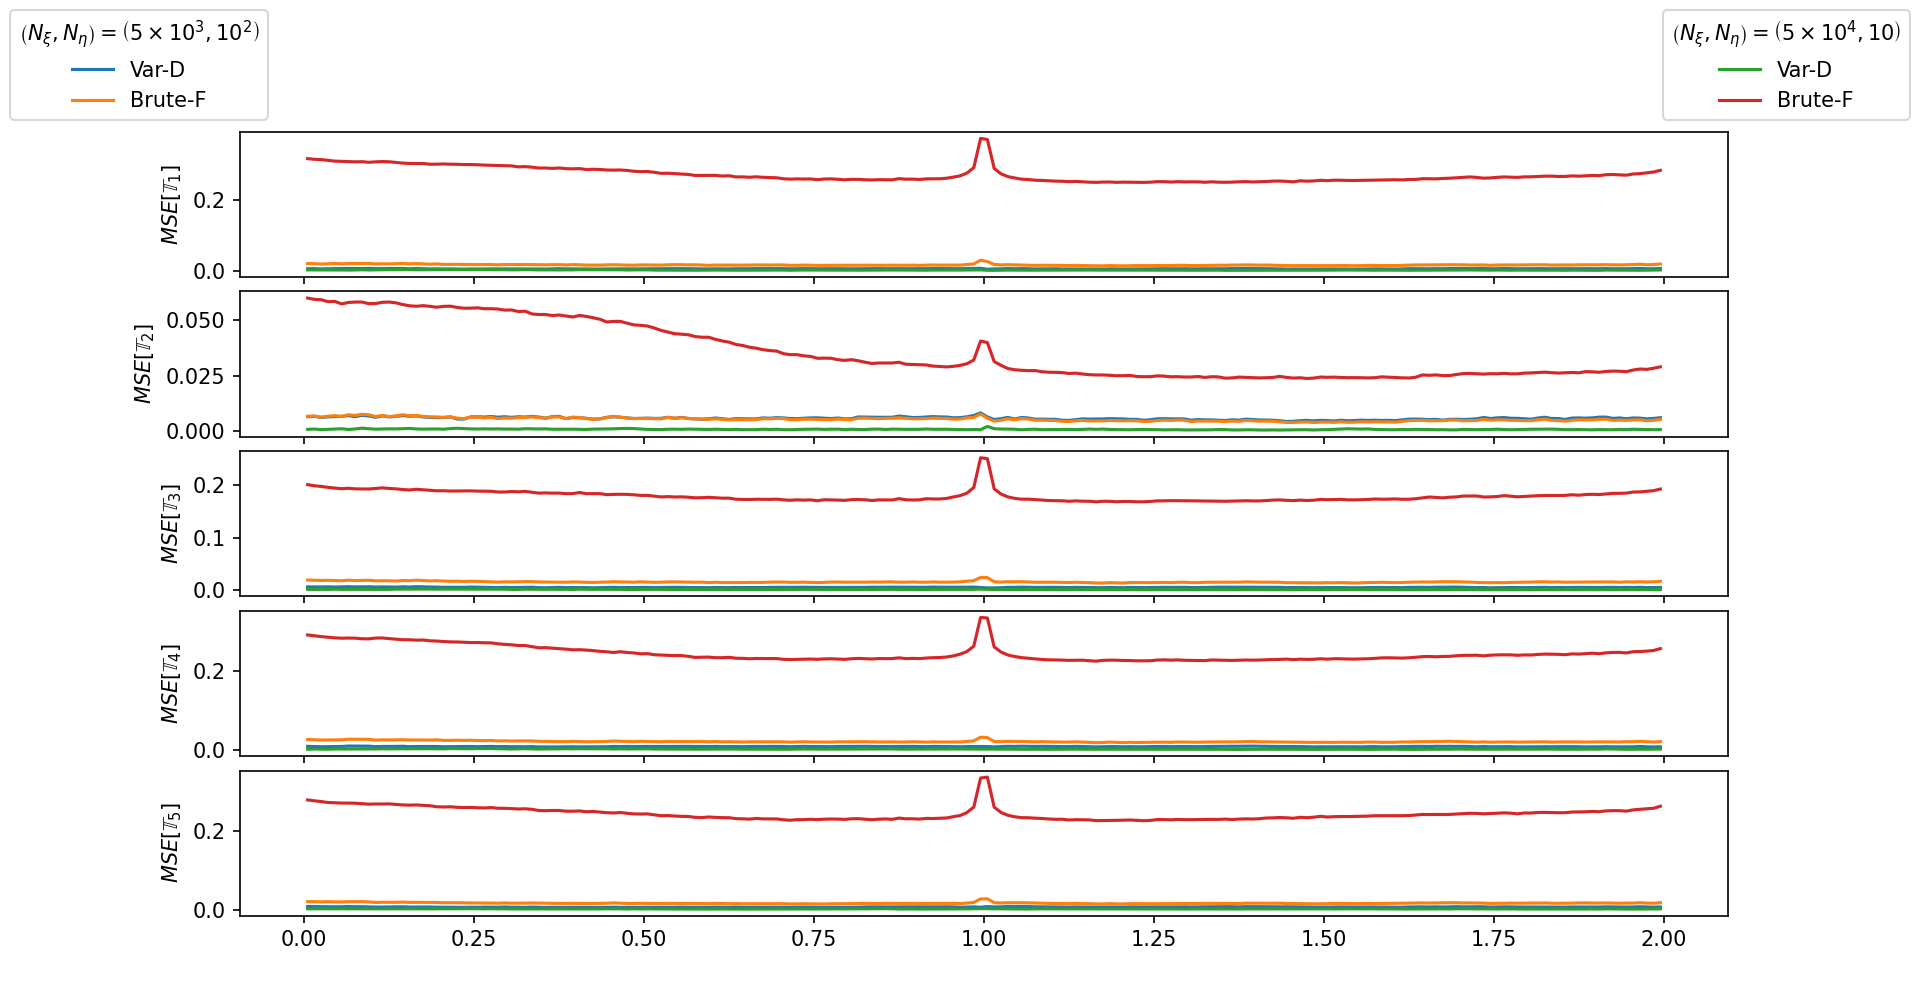
\includegraphics[width=\textwidth]{figures/mse_totalorder_fast.png}
    \caption{$MSE\left[\T{i}\right]$ for $\phi_F$, constant computational cost $\C = \left( \Nxi \times \Neta \right) = 5 \times 10^5$.}
    \label{fig:mse-to-fast}
\end{figure}

\begin{figure}
    \centering
    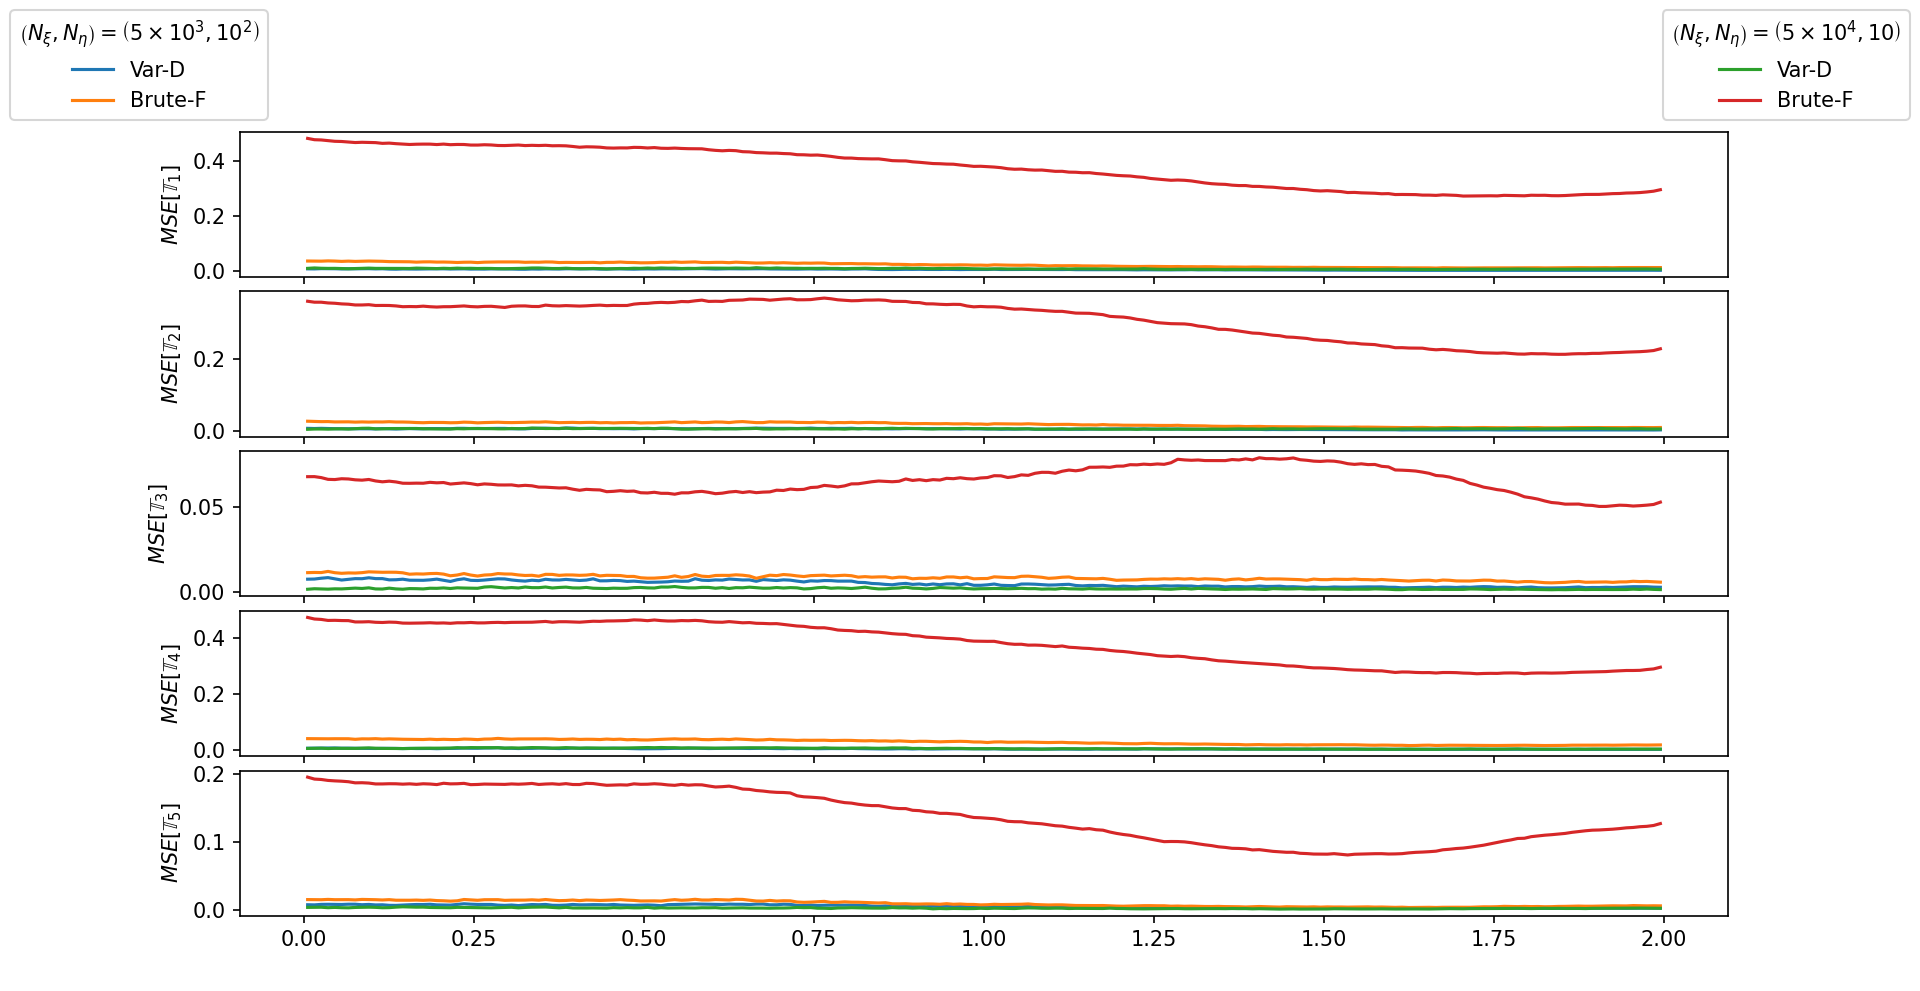
\includegraphics[width=\textwidth]{figures/mse_totalorder_slow.png}
    \caption{$MSE\left[\T{i}\right]$ for $\phi_S$, constant computational cost $\C = \left( \Nxi \times \Neta \right) = 5 \times 10^5$.}
    \label{fig:mse-to-slow}
\end{figure}

We have shown, in this example and the analytic test case, that when increasing computational cost for more accurate estimates of $\S{i}$ and $\T{i}$, putting those computational resources towards increasing $\Nxi$ with the variance deconvolution estimator will improve the accuracy of indices that are not near zero.
